\section{转动和角动量}

\subsection{三维实空间中的转动}

有限大小的物体可以在三维实空间中转动,这是人们的日常经验。现在假设我们研究的是刚体\index{Rigid body:刚体}(Rigid body),即物体的大小、形状及物体各部分与各部分之间的关系都是完全被规定而且是不变的情况。

任意的转动可以被描述为:(1)刚体围绕某个确定的转轴;(2)按右手螺旋转了一个角度。

这两个陈述要拿到一起来看,首先转轴的取向与刚体旋转的方向要构成一个“右手法则”,即右手大拇指的指向要指在转轴的取向上,与此同时右手的其它四个手指自然握紧的方向要与刚体旋转的方向一致。

在这样的约定下,我们需要三个参数来描述刚体的转动,首先转轴的取向需要两个参数,一个是转轴与$z$轴的夹角(polar angel),一个是转轴在$xy$平面上的方位角(azimuthal angel)。

刚体在三维实空间中的转动可以看做是我们施与刚体的一个操作,这个操作被记为$R_{\hat n}(\phi)$,这里单位向量$\hat n$表示转轴的取向,$\phi$表示刚体旋转的角度。

我们可以对刚体施与连续的操作$A$,$B$,这里$A$和$B$表示两个不同的转动,作为一个重要的经验,我们知道转动的后果,与我们实施转动的次序是有关的,用符号的语言表示就是$AB$未必与$BA$相同。

我们知道:如果是定轴转动,转动的效果与转动的次序无关,即$AB = BA$;但如果是定点转动,$A$和$B$两次转动的转轴不在一条直线上,那么$AB$的效果就与$BA$不同。

(这里我们约定转动的次序是从右到左依次进行的,即对依次进行的转动$AB$而言,我们先进行的是$B$操作,然后进行的是$A$操作。)

作为例子我们可以考虑转动$R_x(\frac{\pi}{2})R_z(\frac{\pi}{2})$和$R_z(\frac{\pi}{2})R_x(\frac{\pi}{2})$:

\begin{figure}[htbp]
\begin{center}
\includegraphics[width=9cm]{AngularMomentum/Rotation.png}
\caption{三维实空间中的转动}
%\label{default}
\end{center}
\end{figure}

如图我们用一个带红色箭头的矩形代表刚体,矩形的短边和长边可以区分前后、左右,而附带的红色箭头可用来表示上下。上半图表示的是$R_x(\frac{\pi}{2})R_z(\frac{\pi}{2})$,即先围绕$z$轴转$90^o$再围绕$x$轴转$90^o$,最终结果是红色的箭头向左。下半图是$R_z(\frac{\pi}{2})R_x(\frac{\pi}{2})$,最终的结果是红色箭头向前。即围绕不同转轴的转动操作与实施的次序有关。

对给定刚体,我们可以用某个向量$V$来表示刚体上的任意一点,在转动操作下,向量$V$会变换为$R V$,我们的日常经验告诉我们转动不会改变向量$V$的大小,

\begin{equation}
\left( R V \right)^T RV = V^T R^T R V = V^T V 
\end{equation}

这里$V$是个三维列向量,表示物理空间中的一个向量,$R$是个$3 \times 3$的正交矩阵\index{Orthogonal matrix:正交矩阵}(Orthogonal matrix),即:

\begin{equation}
R^T R = 1
\end{equation}

但其实光这个还不够,因为一般我们不把像空间反演\index{inversion:空间反演}(inversion)或照镜子这样的操作称为转动,比如我们会说在三维实空间中,无论你怎么转动都不能把你的左手转到和你的右手完全“重合”。所以我们还要附加一个条件,就是:

\begin{equation}
\det R = 1
\end{equation}

很容易验证,对空间反演矩阵$i = \left( \begin{array}{ccc} -1 & 0 & 0 \\ 0 & -1 & 0 \\ 0 & 0 & -1 \end{array} \right)$,或一个$x-y$平面上的“照镜子”$ m_{xy} = \left( \begin{array}{ccc} 1 & 0 & 0 \\ 0 & 1 & 0 \\ 0 & 0 & -1 \end{array} \right) $,有$\det i = -1$ 和 $ \det m_{xy} = -1$。

现在我们就可以用一个$\det R = 1$的三维正交矩阵来表示一个三维实空间中的转动。在群论的语言里,我们说这种对转动的表示构成了一个SO(3)群,3表示三维,O表示正交,而S表示“特殊”($\det R = 1$),一个“特殊的三维正交群”。

利用解析几何知识,我们很容易求出$R_z(\phi)$的形式:

\begin{equation}
R_z (\phi) = \left( \begin{array}{ccc} \cos \phi & - \sin \phi & 0 \\ \sin \phi & \cos \phi & 0 \\ 0 & 0 & 1 \end{array} \right)
\end{equation}

类似还可写出$R_x (\phi)$和$R_y (\phi)$(把矩阵中得行和列按规则的方式进行上下和左右的平移,并注意在此过程中保证$\det R = 1$)。

\begin{eqnarray}
R_x (\phi) & = & \left( \begin{array}{ccc} 1 & 0 & 0 \\ 0 & \cos \phi & - \sin \phi \\ 0 & \sin \phi & \cos \phi \end{array} \right) \\
R_y (\phi) & = & \left( \begin{array}{ccc} \cos \phi & 0 & \sin \phi \\ 0 & 1 & 0 \\ - \sin \phi & 0 & \cos \phi \end{array} \right)
\end{eqnarray}

我们特别关心无穷小的转动,这里我们取$\phi = \epsilon$,并对矩阵元进行展开,$\cos \epsilon$没有一阶无穷小,为了得到有意义的结果,我们展开到小量$\epsilon$的二阶。

\begin{equation}
R_z (\epsilon) = \left( \begin{array}{ccc} 1- \frac{\epsilon^2}{2} & - \epsilon & 0 \\ \epsilon & 1- \frac{ \epsilon^2 }{2} & 0 \\ 0 & 0 & 1 \end{array} \right)
\end{equation}

\begin{equation}
R_x (\epsilon) = \left( \begin{array}{ccc} 1 & 0 & 0 \\ 0 & 1- \frac{ \epsilon^2 }{2} & - \epsilon \\ 0 & \epsilon & 1 - \frac{\epsilon^2}{2} \end{array} \right)
\end{equation}

\begin{equation}
R_y (\epsilon) = \left( \begin{array}{ccc} 1- \frac{\epsilon^2}{2} & 0 & \epsilon \\ 0 & 1 & 0 \\  - \epsilon & 0 & 1 - \frac{\epsilon^2}{2} \end{array} \right)
\end{equation}

我们把$R_x(\epsilon)$,$R_y(\epsilon)$代入$R_x (\epsilon) R_y (\epsilon) - R_y (\epsilon) R_x (\epsilon) $中,得到:

\begin{equation*}
\left( \begin{array}{ccc}  0 & - \epsilon^2 & 0 \\  \epsilon^2 & 0 & 0 \\ 0 & 0 & 0 \end{array} \right)
\end{equation*}

即:

\begin{equation}
R_x (\epsilon) R_y (\epsilon) - R_y (\epsilon) R_x (\epsilon) = R_z ( \epsilon^2 ) - 1
\end{equation}

\subsection{对态矢量的无穷小转动}

上一小节我们讨论了对三维实空间中的转动,并得到了一个对转动的数学表示,即用一个行列式为1的三维正交矩阵去表示。这里的转动是针对三维真实物理向量$V$实施的,所谓刚体只不过是无穷多个关系固定的三维向量的集合(当然对每个向量还需附加一个质量密度)。

在量子力学中我们用一个态矢量$\left| \alpha \right\rangle$来描述物理系统的运动状态,态矢量不存在于真实的物理空间,它是数学空间(希尔伯特空间\index{Hilbert Space:希尔伯特空间})中的一个向量。而这个数学空间的维度与真实物理空间的维度是两回事,我们生活的物理世界是三维的,但对希尔伯特空间而言却可以是任意多维的(比如对自旋,我们就用一个二维复线性系数向量空间来描述态矢量)。

我们现在关心的是当物理系统在经历一个真实的转动(用$R$来表示)的同时,描述它的态矢量是如何随之变换的,我们认为会有一个希尔伯特空间中的变换算符($D(R)$)来联系其转动前($\left| \alpha \right\rangle$)和转动后($\left| \alpha \right\rangle_R$)的态矢量:

\begin{equation}
\left| \alpha \right\rangle_R = D(R) \left| \alpha \right\rangle
\end{equation}

这里$D$是德文转动一词“Drehung”的首字母。在三维实空间转动$R$的作用下:

\begin{eqnarray*}
V  &  \xrightarrow {R}  &   RV \\
\left| \alpha \right\rangle   &   \xrightarrow {R}  &  D(R)  \left| \alpha \right\rangle 
\end{eqnarray*}

类似于我们曾经对平移算符和时间演化算符的讨论,我们要求“转动”前的态矢量和“转动”后的态矢量“大小”不变,这要求转动算符$D(R)$是个幺正算符。模仿从前的思路,我们也讨论无穷小转动对应的$D(R)$,它将也被写为:

\begin{equation*}
1 - iG \epsilon
\end{equation*}

的形式,这里$G$是个厄米算符,因此有一个物理量与之对应,在经典物理中与转动对应的物理量是角动量\index{Angular Momentum:角动量}(Angular Momentum),于是我们也称这个物理量为角动量。

这样由旋转对称性的考虑出发,我们就得到了量子力学中角动量的定义,在这个定义中我们并没有用到经典物理中轨道角动量$\vec x \times \vec p$的定义形式,因此这个定义就超出了轨道角动量,把轨道和自旋角动量都放到同一个框架下来研究。

假设转轴的取向是$\hat n$,我们用$J \cdot {\hat n}$来表示延$\hat n$取向的角动量,由于单位选取的缘由,我们用$\frac{J \cdot {\hat n}}{\hbar} \to G$。

无穷小的对态矢量的转动就是:

\begin{equation}
D( R_{\hat n}( d \phi) ) = D (\hat n, \phi) = 1 - i \frac{ J \cdot \hat n}{ \hbar} d \phi
\end{equation}

比如,我们可以写出$D_x (d \phi)$等,

\begin{equation}
D_x(d \phi) = 1 - i \frac{J_x d \phi }{ \hbar }
\end{equation}

在上一小节中我们曾推出对无穷小三维实空间转动$R$存在以下关系:

\begin{equation*}
R_x (\epsilon) R_y (\epsilon) - R_y (\epsilon) R_x (\epsilon) = R_z ( \epsilon^2 ) - 1
\end{equation*}

现在$D(R)$也是对应$R$的,或者说$D(R)$也构成了对旋转$R$的一个表示,$D(R)$应该满足类似的关系:

\begin{equation}
D_x(\epsilon) D_y(\epsilon) - D_y(\epsilon)  D_x(\epsilon)  = D_z(\epsilon^2 ) - 1  
\end{equation}

考虑到等式右侧,

\begin{equation*}
D_z( \epsilon^2 ) = 1 - i \frac{ J_z \epsilon^2 }{ \hbar}
\end{equation*}

我们也需对等式左侧展开到$\epsilon^2$的项。

对有限角度$\phi$的转动而言, 

\begin{equation}
D_x( \phi ) = e^{- i \frac{J_x \phi }{ \hbar }}
\end{equation}

把$D_x( \epsilon )$展开到二阶小量:

\begin{equation}
D_x( \epsilon ) = 1- i \frac{J_x \epsilon }{ \hbar } - \frac{ J_x^2 \epsilon^2  }{2 \hbar^2} + ...
\end{equation}

把以上结果代入$D_x(\epsilon) D_y(\epsilon) - D_y(\epsilon)  D_x(\epsilon)  = D_z(\epsilon^2 ) - 1  $中,左右都表示为二阶小量,整理后可得:

\begin{equation}
[ J_x, J_y ] = i \hbar J_z
\end{equation}

这就是角动量算符的基础对易式\index{fundamental commutation relations of angular momentum:角动量算符的基础对易式}(fundamental commutation relations of angular momentum)。

\subsection{幺正幺模群}

当转动$R$发生时,实空间中的向量$V$按变换$RV$变换,希尔伯特空间中的向量$\left| \alpha \right\rangle$按$D(R) \left| \alpha \right\rangle$变换。

对自旋1/2的粒子,

\begin{equation}
e^{\frac{-i S \cdot n \phi}{\hbar}} = e^{ \frac{ - i \sigma \cdot n \phi }{2} }
\end{equation}


这里$S = \frac{\hbar \sigma}{2} $,$\sigma$是泡利矩阵。这里的$\sigma \cdot n$要理解为$\sigma_n$,即延空间取向$\hat n $的泡利矩阵;同样地,把$S_n$理解为延空间取向$\hat n$的自旋算符(作为特例,自然是$S_x$,延$\hat x$方向的自旋算符,$S_y$,延$\hat y$方向的自旋算符等)。

比如,我们知道$S_z$的本征值问题:

\begin{equation}
S_z \left| + \right\rangle = \frac{\hbar}{2} \left| + \right\rangle
\end{equation}

\begin{figure}[htbp]
\begin{center}
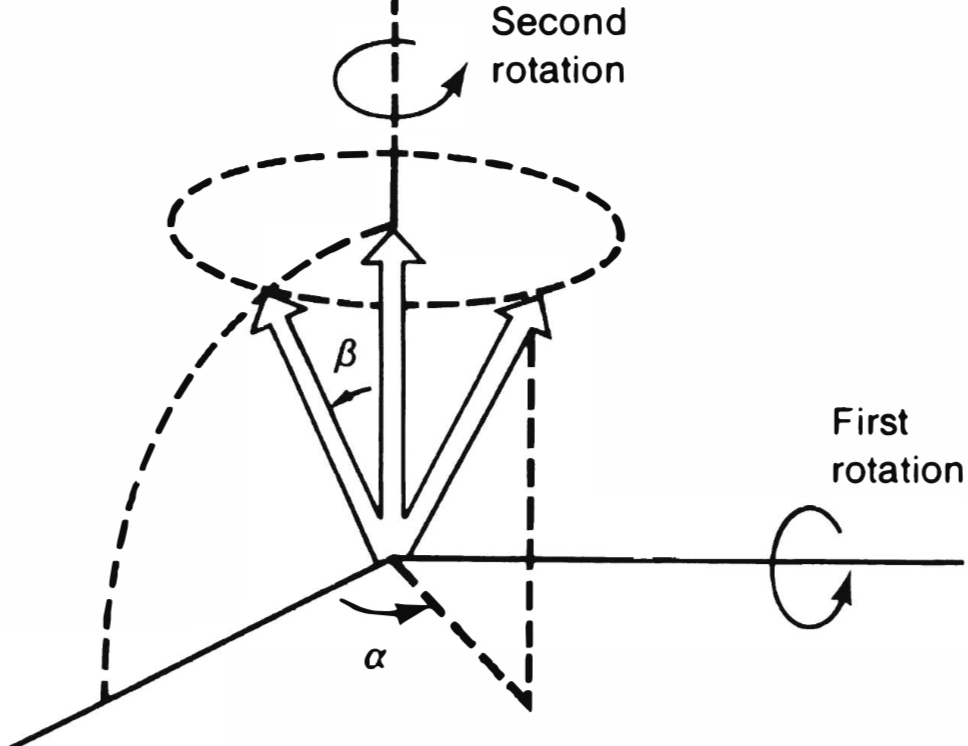
\includegraphics[width=7cm]{AngularMomentum/alphabeta.png}
\caption{倾角$\alpha$和方位角$\beta$的定义。}
%\label{default}
\end{center}
\end{figure}

假设$\hat n$的取向用如图$\alpha$,$\beta$两个角来表示,即$\hat n$的取向由$\hat z$出发,先倒下一个倾角$\alpha$,再在$x-y$平面上转过一个方位角$\alpha$。

$S_n$是延$\hat n$方向的,其本征值问题是:

\begin{equation}
S_n \left| n,+ \right\rangle = \frac{\hbar }{2} \left| n,+ \right\rangle
\end{equation}

这里的$\left| n,+ \right\rangle$可看做是对$S_z$的本征矢$\left| + \right\rangle$先围绕$y$轴转$\beta$角度,再围绕$z$轴转$\alpha$角度。

\begin{equation}
\left| n,+ \right\rangle = e^{- \frac{ i S_z \alpha }{ \hbar }}  e^{- \frac{ i S_y \beta }{ \hbar }}  \left| + \right\rangle
\end{equation}

这里我们规定:$U = e^{- \frac{ i S_z \alpha }{ \hbar }}  e^{- \frac{ i S_y \beta }{ \hbar }}$。

$S_z$的本征值问题可改写为:

\begin{equation}
U S_z U^\dagger U \left| + \right\rangle = \frac{\hbar}{2} U \left| + \right\rangle
\end{equation}

即:

\begin{equation}
S_n = U S_z U^\dagger
\end{equation}

或改写为泡利矩阵的形式:

\begin{equation}
\sigma_n = U \sigma_z U^\dagger
\end{equation}

即:

\begin{equation}
\sigma_n = e^{- \frac{ i \sigma_z \alpha }{2}} e^{- \frac{ i \sigma_y \beta }{2}} \sigma_z e^{ \frac{ i \sigma_y \beta }{2}}  e^{ \frac{ i \sigma_z \alpha }{2}}
\end{equation}

展开后可得:

\begin{equation}
\sigma_n = \left( \begin{array}{cc}  \cos \beta & \sin \beta e^{- i \alpha}  \\  \sin \beta e^{i \alpha} & - \cos \beta  \end{array}  \right)
\end{equation}

在$\hat n$方向旋转$\phi$角度的变换矩阵为:

\begin{equation}
e^{- \frac{ i \sigma_n \phi}{2}} = 1 \cos \left( \frac{\phi}{2} \right) - i \sigma_n \sin \left( \frac{\phi}{2}  \right) 
\end{equation}

上式中的$1$表示单位算符,计算可得:

\begin{equation}
e^{- \frac{ i \sigma_n \phi}{2}} = \left( \begin{array}{cc}   \cos \frac{\phi}{2} - i \cos \beta \sin \frac{\phi}{2} & - i \sin \beta e^{- i \alpha} \sin \frac{\phi}{2} \\  - i \sin \beta e^{i \alpha} \sin \frac{\phi}{2} & \cos \frac{\phi}{2} + i \cos \beta \sin \frac{\phi}{2}   \end{array}  \right)
\end{equation}

考虑到单位向量$\hat n$在$x$, $y$和$z$轴的投影:

\begin{eqnarray}
n_x & = & \sin \beta \cos \alpha \\
n_y & = & \sin \beta \sin \alpha \\
n_z & = & \cos \beta
\end{eqnarray}

$e^{- \frac{ i \sigma_n \phi}{2}}$可表示为:

\begin{equation}
e^{- \frac{ i \sigma_n \phi}{2}} = \left( \begin{array}{cc}   \cos \frac{\phi}{2} - i n_z \sin \frac{\phi}{2} & \left( - i n_x - n_y  \right) \sin \frac{\phi}{2} \\  \left( - i n_x + n_y  \right) \sin \frac{\phi}{2} & \cos \frac{\phi}{2} + i n_z \sin \frac{\phi}{2}   \end{array}  \right)
\end{equation}

所有这样的操作构成了一个幺正幺模群\index{Unitary unimodular group:幺正幺模群}(Unitary unimodular group),幺正条件是$U^\dagger U = 1$,幺模条件是$\det U = 1$(泡利矩阵$\sigma_x$等就不满足幺模条件)。

一个二维幺正幺模的矩阵可表示为:

\begin{equation}
U(a,b)=\left( \begin{array}{cc}  a & b \\ - b^* & a^*  \end{array} \right)
\end{equation}

同时必须满足:

\begin{equation}
|a|^2 + |b|^2 = 1
\end{equation}

我们把二维的幺正幺模群记为SU(2),这里的S表示Special。值得注意的是,尽管SU(2)和SO(3)都可用以表示三维实空间中的转动,但它们并不是同构的(isomorphic)。考虑一个$\phi = 2 \pi$的旋转和一个$4 \pi$的旋转,对SO(3)我们得到相同的矩阵元,但对SU(2)则正好差一个负号,但我们可以构造U(a,b)或U(-a,-b)到SO(3)的一一对应,在此意义上我们说它们是局域同构的(locally isomorphic)。

\subsection{欧拉转动}

三维实空间(物理空间)中的转动可以用三个参量来表示(比如$\hat n (\beta, \alpha)$和$\phi$),我们也可以用欧拉转动\index{Euler Rotations:欧拉转动}(Euler Rotations)来表示。

欧拉转动($\alpha, \beta, \gamma$)的定义如图:

\begin{figure}[htbp]
\begin{center}
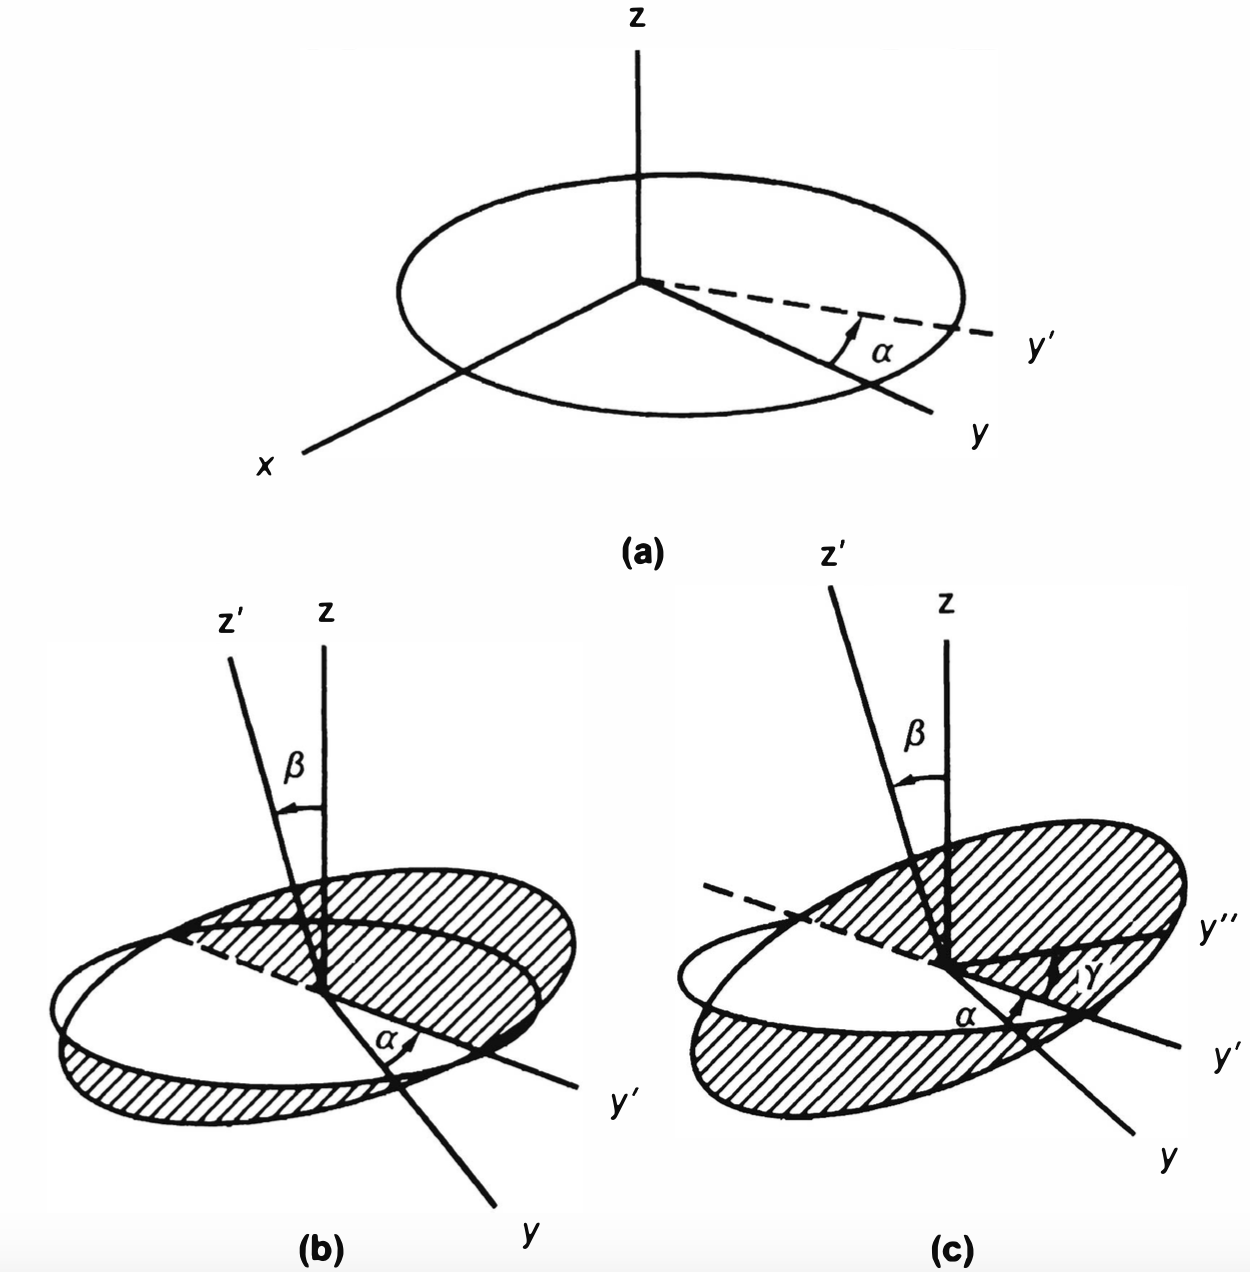
\includegraphics[width=10cm]{AngularMomentum/eulerrotations.png}
\caption{欧拉转动}
%\label{default}
\end{center}
\end{figure}

首先我们要注意区分两种坐标系,一种是空间固定的(space-fixed)坐标系,用$O-xyz$表示,另一种是物体固定的(body-fixed)坐标系,用$O-x' y' z'$等表示。

欧拉转动$R(\alpha, \beta, \gamma)$被定义为(a)围绕空间固定的$z$轴转$\alpha$角;然后(b)围绕物体固定的$y'$轴转$\beta$角,注意此时$y'$轴和空间固定的$y$轴已经不重合了,相差有$\alpha$角;最后(c)围绕物体固定的$z'$轴转$\gamma$角,这个$z'$轴和$z$轴相差$\beta$角。

\begin{equation}
R(\alpha, \beta, \gamma) = R_{z'}(\gamma) R_{y'} (\beta) R_z (\alpha)
\end{equation}

可以验证各个转动间存在着这样的关系:

\begin{equation}
R_{y'}(\beta) = R_z (\alpha) R_y (\beta) R_z^{-1}(\alpha)
\end{equation}

这里$R^{-1}$表示“反方向”转,通过使一个扁平物体按步骤转起来不难证明以上关系。类似地,我们还有:

\begin{equation}
R_{z'}(\gamma) = R_{y'} (\beta) R_z (\gamma) R_{y'}^{-1}(\beta)
\end{equation}

由以上两个关系,我们可以证明:

\begin{eqnarray*}
R_{z'} (\gamma) R_{y'} (\beta) R_z (\alpha) & = &  R_{y'} (\beta) R_z (\gamma) R_{y'}^{-1}(\beta) R_{y'} (\beta) R_z (\alpha) \\
{} & = & R_{y'} (\beta) R_z (\gamma) R_z (\alpha) \\
{} & = & R_z (\alpha) R_y (\beta) R_z^{-1}(\alpha) R_z (\gamma) R_z (\alpha) \\
{} & = & R_z (\alpha) R_y (\beta) R_z (\gamma)
\end{eqnarray*}

由以上关系,我们可得到在态空间中转动的算符的关系:

\begin{equation}
D(\alpha, \beta, \gamma ) = D_z (\alpha) D_y (\beta) D_z (\gamma)
\end{equation}

现在所有转动($\alpha$,$\beta$和$\gamma$)都是针对空间固定的转轴进行的。

\subsection*{参考}

J. J. Sakurai, Modern Quantum Mechanics, \S 3.1, 3.2, 3.3

